\PassOptionsToPackage{unicode}{hyperref}
\documentclass[aspectratio=1610, professionalfonts, 9pt]{beamer}

\usefonttheme[onlymath]{serif}
\usetheme[showtotalframes]{tudo}

\ifluatex
  \usepackage{polyglossia}
  \setmainlanguage{german}
\else
  \ifxetex
    \usepackage{polyglossia}
    \setmainlanguage{german}
  \else
    \usepackage[german]{babel}
  \fi
\fi

\newcommand*\xRightarrow[2][]{\ext@arrow 0359\Rightarrowfill@{#1}{#2}}

% Mathematik
\usepackage{amsmath}
\usepackage{amssymb}
\usepackage{mathtools}
\usepackage{cancel}

\usepackage{hyperref}
\usepackage{bookmark}
\usepackage{siunitx}
%%%%%%%%%%%%%%%%%%%%%%%%%%%%%%%%%%%%%%%%%%%%%%%%%%%%%%%%%%%%%%%%%%%%%%%%%%%%%%%%
%%%%%-------------Hier Titel/Autor/Grafik/Lehrstuhl eintragen--------------%%%%%
%%%%%%%%%%%%%%%%%%%%%%%%%%%%%%%%%%%%%%%%%%%%%%%%%%%%%%%%%%%%%%%%%%%%%%%%%%%%%%%%

%Titel:
\title{Stromnetz und Strombörse}
%Autor
\author[D.~Hering]{Dag-Björn Hering}
%Lehrstuhl/Fakultät
%\institute[Experimental Physics 5]{Names des Lehrstuhls \\  Name der Fakultät}
%Titelgrafik
\titlegraphic{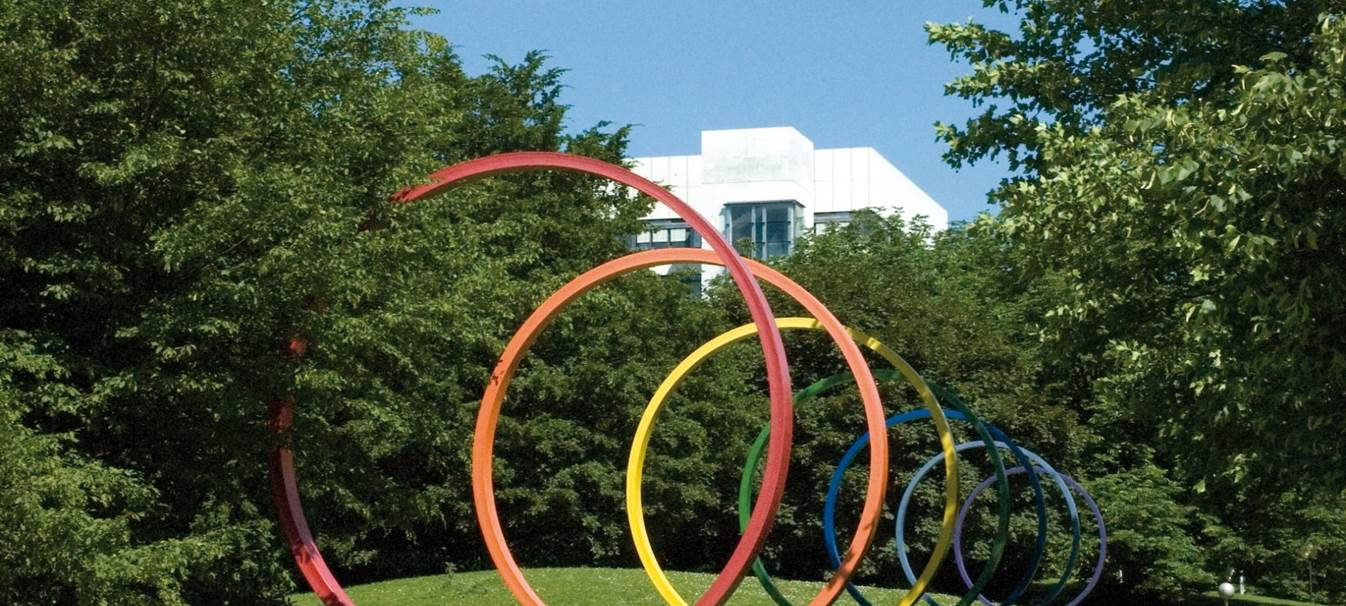
\includegraphics[width=0.7\textwidth]{images/tudo-title-2.jpg}}


\begin{document}
\maketitle
\begin{frame}
\end{frame}

\begin{frame}{Gliederung}
\begin{itemize}
  \item Stromnetz
  \begin{itemize}
  \item Vorderungen an das Stromnetz
  \item Frequenz im Netz
  \item Reguationsmechanismen der Frequenz
  \item Spannungsebenen
  \item Verteilung
  \item Netzbetreiber
  \item Anspruch an das Stromnetz durch die Energiewende
  \end{itemize}
\end{itemize}
\end{frame}
\begin{frame}
\begin{itemize}
 \item Strombörse
\begin{itemize}
  \item Enwicklung der Strombörse
  \item Angebote der Strombörse
  \item Spot Markt(und seine Folgen auf das Netz)
  \item Strompreis aus der Merit Order
  \item EEG-Umlage
  \item Strompreisentwicklung
\end{itemize}
\end{itemize}
\end{frame}



{
\setbeamertemplate{footline}{}
\begin{frame}{Europäisches Verbundsystem}
\begin{columns}
\begin{column}{0.5\textwidth}
\begin{itemize}
  \item ensteht aus mehrere von einander getrennte Verbundsysteme
\item Verbundsystem
Zusammenschluss von Höchst und Hochspannungsnetzen der Länder zur z.B. UCT  (Union for the Co-ordination of the Transmission of Electricity)
  \item Verband Europäischer Übertragnungsnetzbetreiber
   European Network of Transmission System (ENTSO-E) übernimmt Koorodination
der Verbundsysteme
\end{itemize}
\end{column}
\begin{column}{0.5\textwidth}
    \begin{figure}
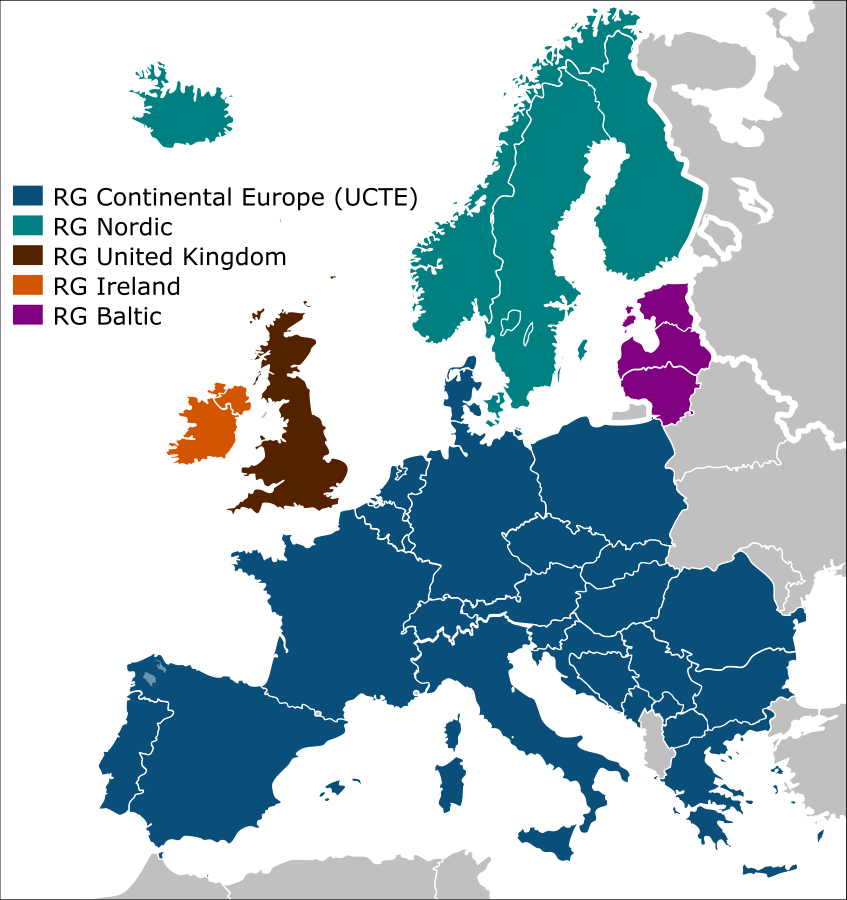
\includegraphics[width=0.9\textwidth]{images/Euronetz.png}
\end{figure}
\end{column}
\end{columns}
% Quelle: https://commons.wikimedia.org/w/index.php?curid=1387849
\end{frame}
}

{
\setbeamertemplate{footline}{}
\begin{frame}
  \begin{columns}
  \begin{column}{0.5\textwidth}
%\frametitle{Netzebenen}
\begin{itemize}
  \item Höchstspannung $\num{380}$/$\SI{220}{\kilo\volt}$
  \item Hochspannung  $\SI{110}{\kilo\volt}$
  \item Mittelspannung  $\num{30}$/$\num{20}$/$\SI{10}{\kilo\volt}$
  \item Niederspannung $\num{230}$/$\SI{400}{\volt}$
\end{itemize}
\end{column}
\begin{column}{0.5\textwidth}
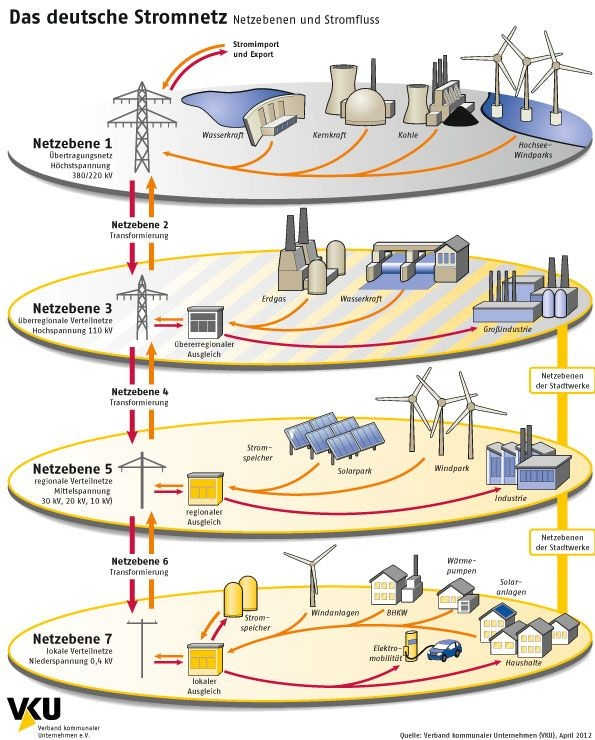
\includegraphics[width=1\textwidth]{images/netzebenen.jpg}
%Quelle: http://www.bpb.de/politik/wirtschaft/energiepolitik/148524/ausbau-des-stromnetzes
\end{column}
\end{columns}
\end{frame}


\begin{frame}
\begin{figure}
  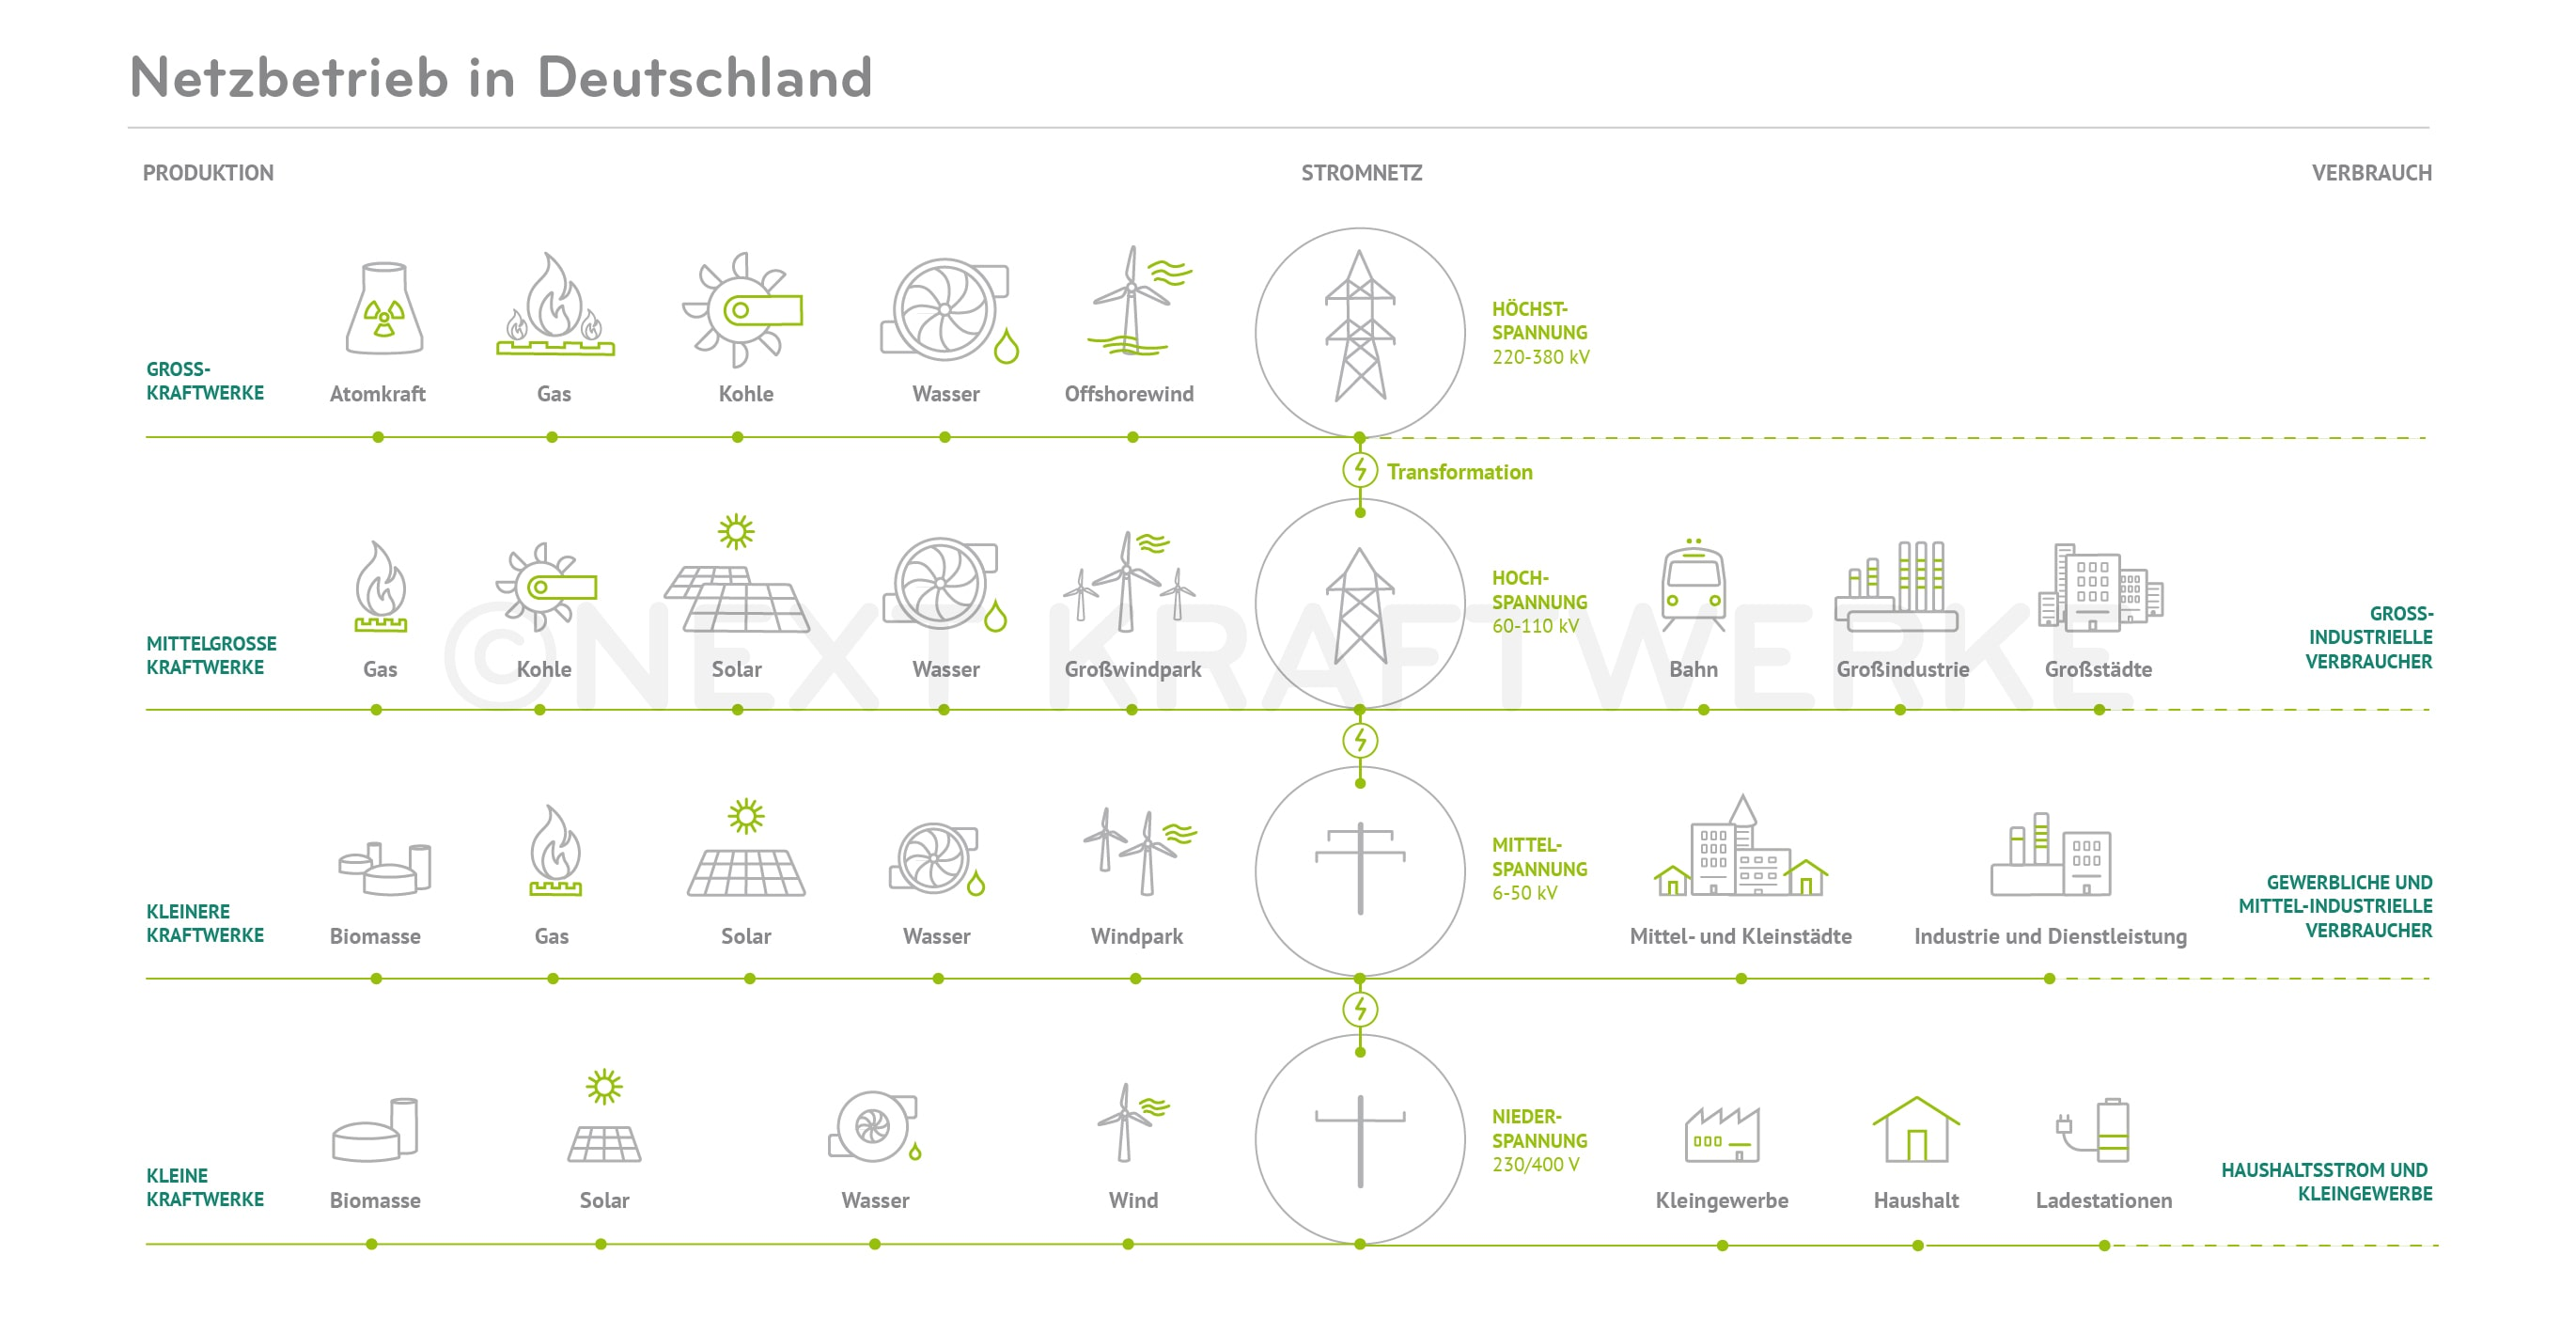
\includegraphics[width=1\textwidth]{images/netzbetrieb-deutsches-stromnetz.jpg}
\end{figure}
%:Quelle:
\end{frame}
}

\begin{frame}
  \begin{columns}
    \begin{column}{0.5\textwidth}
  \begin{itemize}
    \item Hoch-/Mittel-/Niederspannungs Ebenen
     werden regional und lokal von Verteilernetzbetreibern verwaltet
    \item Die Höchstspannung Ebene teilen sich in
    Deutschland die Übertragungsnetzbetreiber
    \begin{itemize}
      \item[-] Tennet
      \item[-] 50-Hertz
      \item[-] Amprion
      \item[-] Transnet
  \end{itemize}
\end{itemize}
\end{column}
\begin{column}{0.5\textwidth}
\begin{figure}
    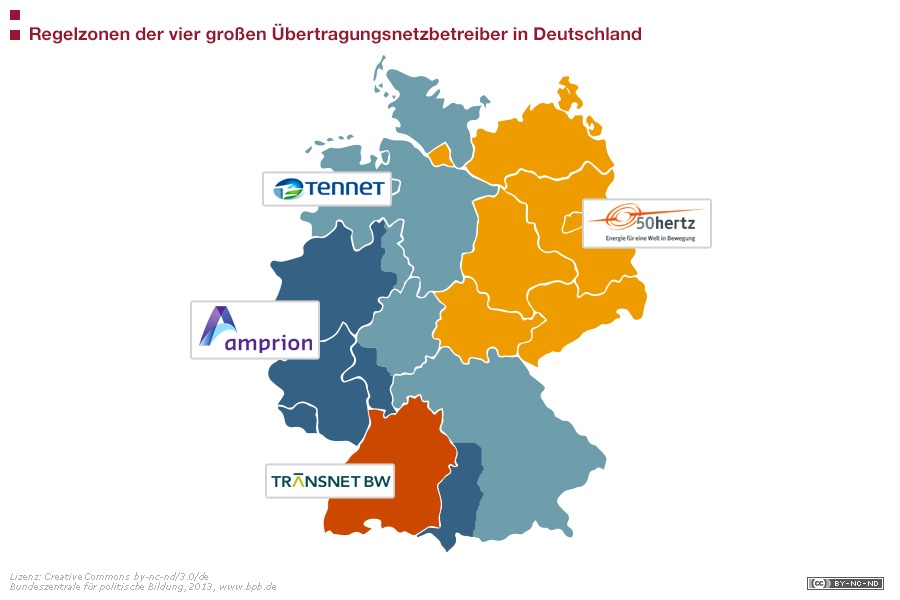
\includegraphics[width=1\textwidth]{images/UNB.jpg}
%Quelle:http://www.bpb.de/politik/wirtschaft/energiepolitik/148524/ausbau-des-stromnetzes
\end{figure}
\end{column}
\end{columns}
\end{frame}

\begin{frame}{Netzfrequenz}
\begin{itemize}[<+->]
\item Richtfrequenz von $\SI{50}{\hertz}$ im Europäischen Verbundnetz
\item Hängt von Rotationsgeschwindigkeit der Synchronisierten Generatoren zusammen\\
Generatoren ab
% Um dieses umgangssprachlicher zu erklären, wird
% gerne der Alltagsvergleich mit einem Fahrrad herangezogen:
% Auf einer gleichmässigen Fläche kann relativ einfach eine
% konstante Trittgeschwindigkeit gehalten werden.
% An einer Steigung (zu vergleichen mit steigender Last im Stromnetz)
% muss mehr Kraft aufgewendet werden, um die Trittfrequenz
% beizubehalten oder sie kann sogar (kurzeitig) sinken,
% bis man sich auf die Steigung eingestellt hat.
% Anders herum steigt die (Tritt-)Frequenz an einem Gefälle
% kurz an, bis man sie (zum Beispiel durch Bremsen) wieder
% auf die „normale“ Nennfrequenz gesenkt hat.
\item Zu starke Abweichungen können Zerstörung der Generatoren und anderen Geräten führen.
% \begin{itemize}[<+->]
%   \item test ...
%   \item test 2
% \end{itemize}
führen
\item Abweichungen in der Frequenz entstehen durch Schwankungen
der Relation von abgenommener und erzeugter Leistung.
\end{itemize}
\end{frame}

{
\setbeamertemplate{footline}{}
\begin{frame}
  \begin{figure}
  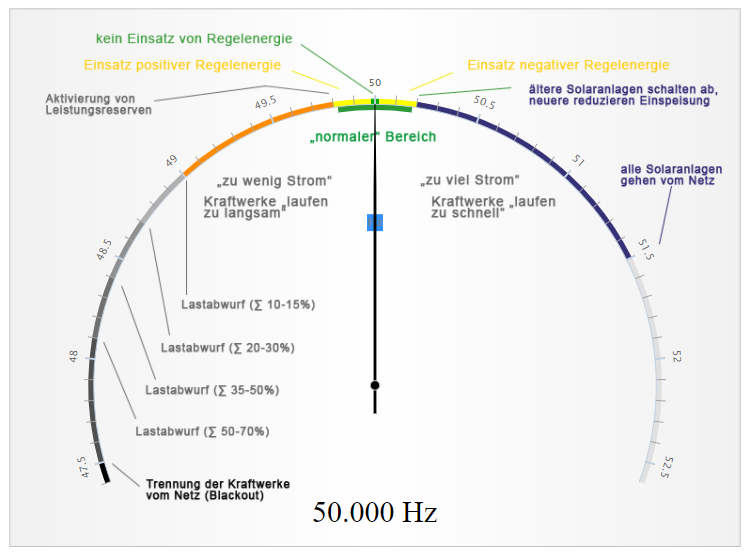
\includegraphics[width=0.9\textwidth]{images/Frequenz.png}
  \end{figure}
%Quelle:http://www.netzfrequenz.info/aktuelle-netzfrequenz-full
\end{frame}
}

\begin{frame}{Regelung der Netzfrequenz}
Notwendigkeit von Regelbarer Leistung um Frequenz konstant zu halten
\begin{itemize}
\item Primärregelung
  \begin{itemize}
    \item[-] automatische vollständige Aktivierung innerhalb von \SI{30}{\second}
    \item[-] Abdeck Zeitraum \num{0}<\SI{15}{\minute}
    \item[-] Bereitstellung durch alle ÜNB im ENTSO-E-Gebiet
  \end{itemize}
\item Sekundärregelung
\begin{itemize}
\item[-] automatische Aktivierung innerhalb von \SI{5}{\minute}
\item[-] ...
\end{itemize}
\item Tertiärregelung(Minutenreserve)
\begin{itemize}
  \item[-] Aktivierung innerhalb von \SI{15}{\minute}
  \item[-] Abdeck Zeitraum mehrere Stunden bei Störungen
\end{itemize}
\end{itemize}
\end{frame}

{
\setbeamertemplate{footline}{}
\begin{frame}
  \begin{figure}
  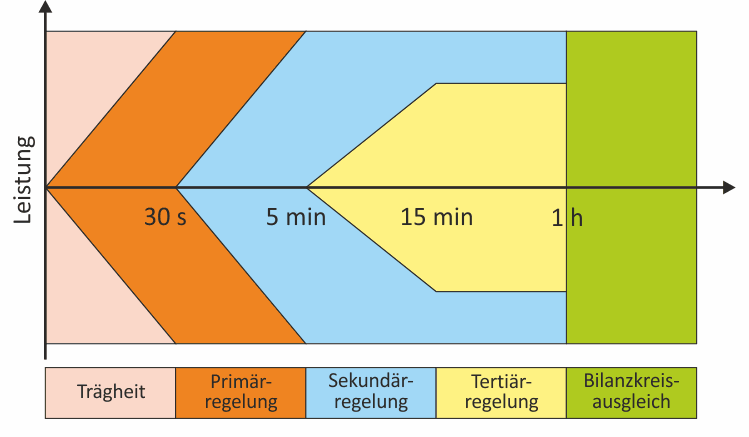
\includegraphics[width=0.9\textwidth]{images/Regelleistung.png}
\end{figure}
%Quelle:https://fenecon.de/page/stromspeicher-energy-pool
\end{frame}
}

\begin{frame}{Energiewende und folgen im Stromnetz}
  \begin{columns}
  \begin{column}{0.5\textwidth}
Konventionelles Stromnetz:
\begin{itemize}
  \item Kraftwerkleistungen werden an Lastprofil angepasst
  \item "Einbahnstraße im Stromnetz" Kraftwerk$\rightarrow$Verbraucher
Höchspannung$\rightarrow$Niederspannung
\end{itemize}
  \end{column}
  \begin{column}{0.5\textwidth}
Neues Stromnetz:
\begin{itemize}
\item EE-Kraftwerkleistungen nur noch bedingt (z.B Wasser) oder garnicht (z.B Wind/Sonne) steuerbar\\$\rightarrow$ somit keine Anpassungs an Lastprofil möglich
\item Durch Erneuerbarenenergien Höchstspannung$\leftrightarrows$Niederspannung
\end{itemize}
\end{column}
\end{columns}
\end{frame}


\begin{frame}{Blackout}
!!!!!!!!!!!!!!!!!!!!!!!!!!!!!!!!!!1
\end{frame}




\begin{frame}{Strombörse}
\begin{itemize}
  \item Standort der European Energy Exchange (EEX) in Leipzig
\item irgendwas mit paris
  \item Stromhandel seit \num{2000}
  \item Nicht nur Handel von Strom sondern auch allen Energie Produkte wie (...)
  \item Unterscheidung zwischen Spotmarkt und Terminmarkt
\end{itemize}
\end{frame}

\begin{frame}{Spotmarkt}
\begin{itemize}
\item Spotmarkt in Paris and der EXAA
\item Handel von kurzfristig lieferbaren Strommengen
\item Im Intraday-Handel (Lieferung am Selbentag)
\item Im Day-Ahead-Handel (Lieferung am Folgetag)
\end{itemize}
\end{frame}

{
\setbeamertemplate{footline}{}
\begin{frame}
  \begin{figure}
  \includegraphics[width=1.1\textwidth]{images/stromprodukte.jpg}
\end{figure}
%Quelle:https://www.next-kraftwerke.de/wissen/strommarkt/spotmarkt-epex-spot
\end{frame}
}

\begin{frame}{Merit-Order}
\begin{itemize}
  \item Beschreibungsmodell der Preisbildung auf dem Strommarkt
  \item orientiert sich an den Grenzkosten der Kraftwerke
  (Grenzkosten enspricht kosten für die letzte produzierte Megawattstunde)
\item Kraftwerke mit niedrigen Grenzkosten werden bei der
 Einspeisung bevorzugt bis Nachfrage gedeckt ist.
\item Börsenpreis ergibt sich aus schnittstelle von Angebot und Nachfrage
\begin{itemize}
  \item[$\rightarrow$] Grenzkosten des Kraftwerkes, welches zuletzt den
  Zuschlag zur Einspeisung erhält, definiert Börsenpreis für alle eingespeisten Kraftwerke("uniform pricing")
\end{itemize}
\end{itemize}
\end{frame}

{
\setbeamertemplate{footline}{}
\begin{frame}
  \begin{figure}
  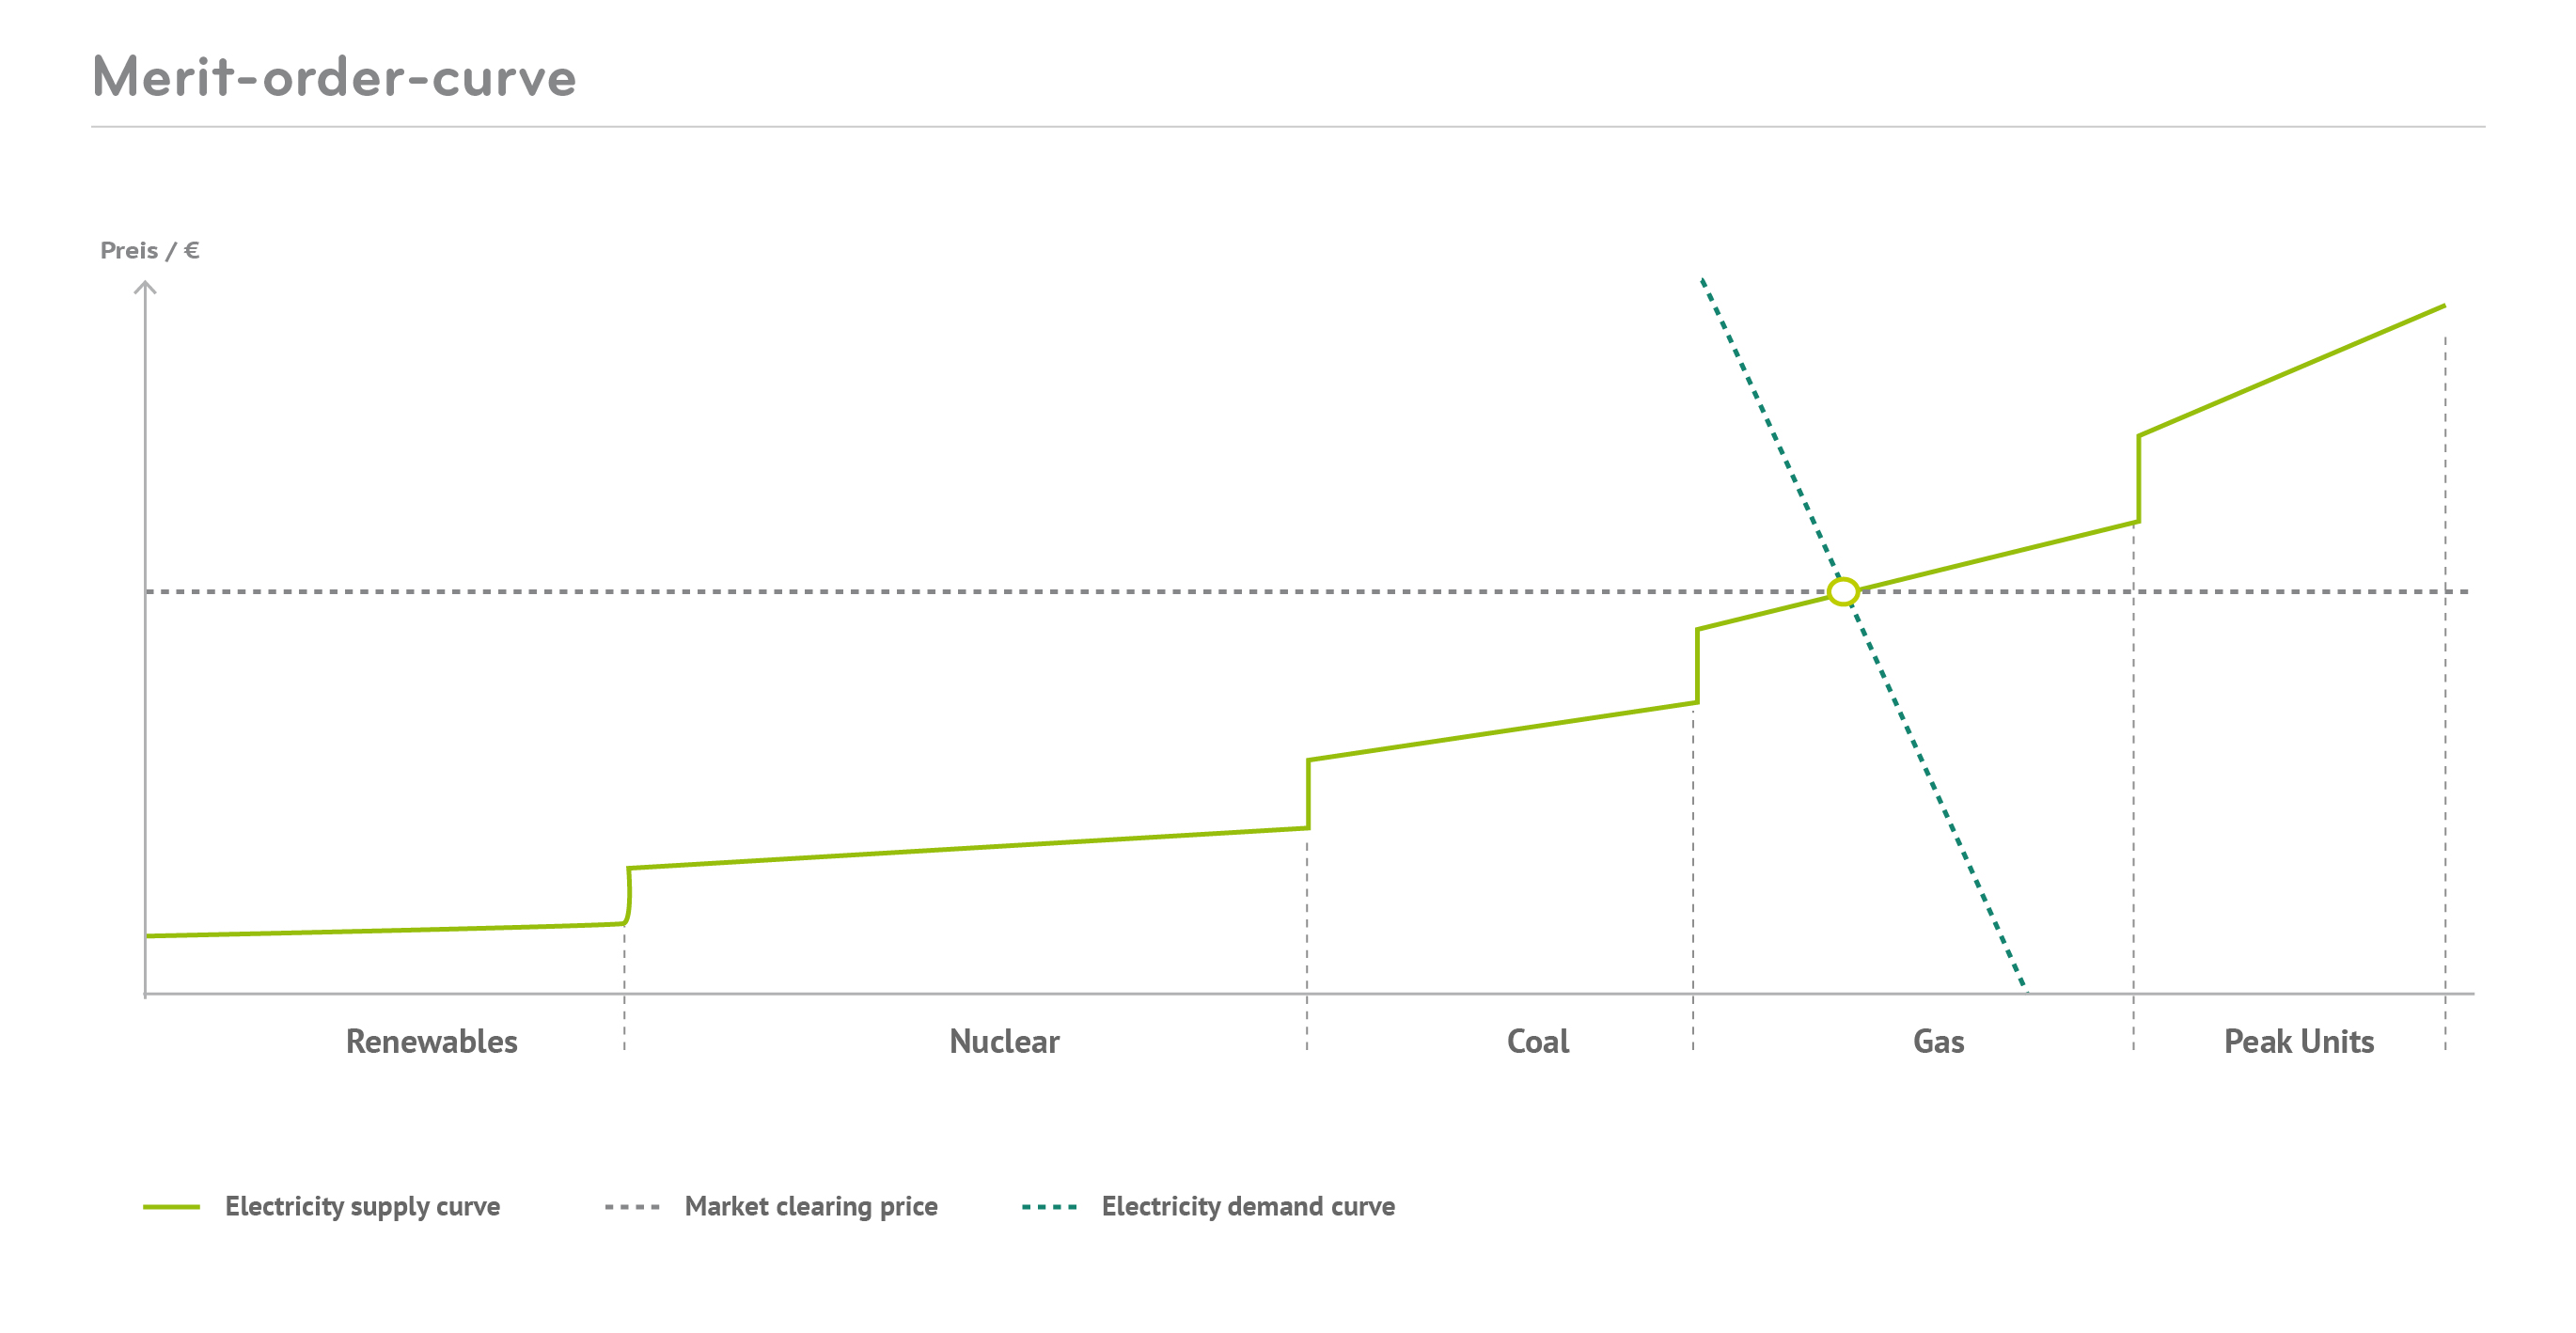
\includegraphics[width=1\textwidth]{images/Merit-order-curve-2.jpg}
\end{figure}
%Quelle:https://www.next-kraftwerke.be
\end{frame}
}

{
\setbeamertemplate{footline}{}
\begin{frame}
  \begin{figure}
  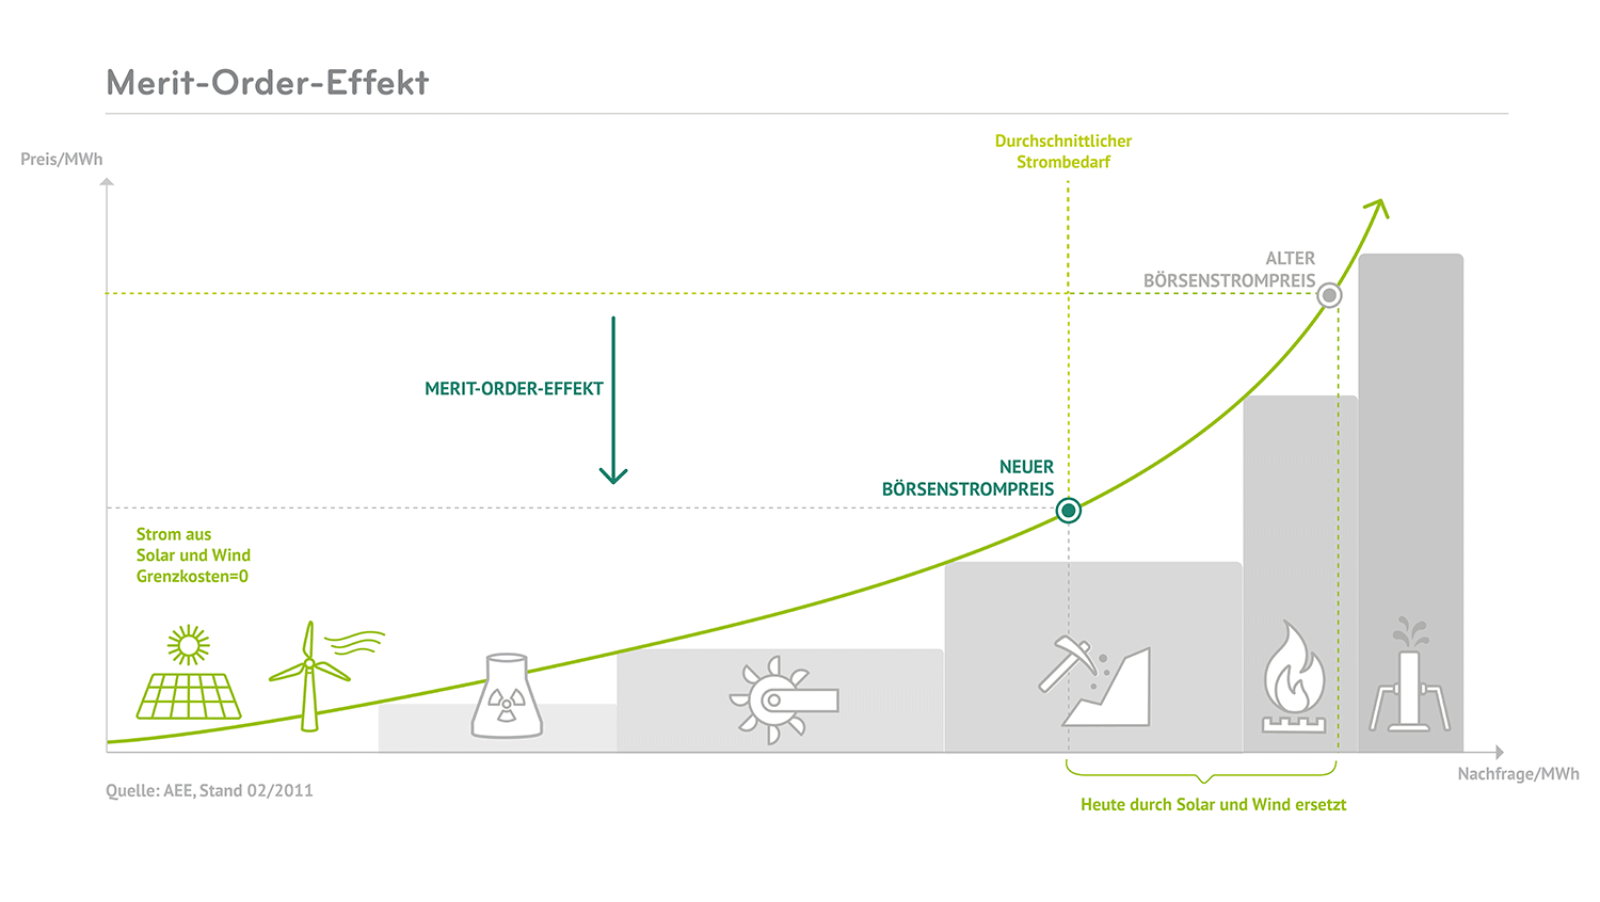
\includegraphics[width=1\textwidth]{images/Merit.png}
\end{figure}
%Quelle:https://www.next-kraftwerke.be
\end{frame}
}

\begin{frame}{Terminmarkt}
\begin{itemize}
  \item Handel von Strommengen, die zu einem festen Termin zu verfügung gestellt werden (Strom-Futures)
  \item bis zu 6 Jahre Strom im vorraus Kaufen
  \item Jahr-, Quatal-, Monat-, Woche-,  Wochenende- und Tagkontrakt
  \item Preis richtig sich an den Börsenindex der Strombörse Phelix (Physical Electricity Index)
\end{itemize}
\end{frame}

\begin{frame}{Erneuerbare-Energie-Gesetz EEG}
   \begin{itemize}
     \item Regelt die Einspeisung des EE-Stromes
     \item Verpflichtung an die Netzbetreiber EE-Strom vorrangig in das Stromnetz einzuspeisen 
   \end{itemize}
\end{frame}

\begin{frame}{Entwicklung}

\end{frame}
\end{document}


\begin{frame}{Paradigmenwechsel}

\end{frame}
